\documentclass[12pt,titlepage]{article}

%% THE USEPACKAGES NECESSARY FOR THIS EXAMPLE
%% NOTE THAT genetics_manu_style MUST BE CALLED AFTER mychicago
\usepackage{graphicx}
%\usepackage{endfloat}
\usepackage{amsfonts}
\usepackage{amsmath}
\usepackage{mychicago}
\usepackage{subfigure}
%\usepackage{genetics_manu_style}
\usepackage{ctable}
\usepackage{lscape}
\usepackage{multirow}

\usepackage{lineno}

%\linespread{2.0}


%% THE MANUSCRIPT TITLE
\title{Corrected Abstract for: Dissecting high-dimensional traits with Bayesian sparse factor analysis of genetic covariance matrices }





%%  THE AUTHOR DECLARATIONS.  USE \THANKS TO GIVE ADDRESSES
\author{Daniel E. Runcie, Sayan Mukherjee}

%% SOME COMMANDS FOR THE CONTENT OF THIS FILE.  NOT NECESSARY FOR
%% GENETIC_MANU_STYLE
\newcommand{\bm}{\mathbf}
\newcommand{\LLL}{\mathcal}




%% BEGIN DOC
\begin{document}


\maketitle
%\linenumbers

\section{Appendix}
\subsection{Posterior sampling:}\label{postsamp}
We estimate the posterior distribution of the Bayesian genetic sparse
factor model with an adaptive partially collapsed Gibbs sampler \cite{vanDyk:2011vb} based on the procedure proposed 
by \citeN{Bhattacharya:2011gh}. The value $k^*$ at
which columns in $\mathbf{\Lambda}$ are truncated is set using
an adaptive procedure \cite{Bhattacharya:2011gh}.
Given a truncation point, the following conditionally posterior distributions are sampled from in order:

\begin{enumerate}

\item 
\label{step:lambda}
The full conditional posterior distribution of the truncated factor loading matrix $\mathbf{\Lambda}_{k^*}$ is dependent on the parameters $\mathbf{B}, \; \mathbf{E}_a, \;\mathbf{F} = \mathbf{Z} \mathbf{F}_a + \mathbf{F}_r$, and $\mathbf{\Psi}_r = \mbox{Diag}(\psi_{r_j})$. The full density factors into independent multivariate normal densities (MVNs) for each row of $\mathbf{\Lambda}_{k^*}$:
\begin{align*}
\pi(\pmb{\lambda}_j \mid \mathbf{y}_j, \; \mathbf{b}_j, \; \mathbf{e}_{a_j}, \;  \; \mathbf{F}, \; \psi_{r_j})
\sim \mbox{N}(\psi^{-1}_{r_j}\mathbf{C}^{-1}\mathbf{F}^T(\mathbf{y}_j - \mathbf{X}\mathbf{b}_j - \mathbf{Z} \mathbf{e}_{a_j}),\mathbf{C}^{-1}),
\end{align*}
\noindent where: $\mathbf{C} = \psi^{-1}_{r_j}\mathbf{F}^T\mathbf{F} + \mbox{Diag}(\psi^{-1}_{jl}\tau^{-1}_j)$.

To speed up the MCMC mixing, we partially collapse this Gibbs update step by marginalizing over $\mathbf{E}_a\sim \mbox{N}(\mathbf{0},\mathbf{A},\mathbf{\Psi}_a)$. Let $\mathbf{\Psi}_a = \mbox{Diag}(\psi_{a_j})$:
\begin{align*}
\pi_{/\mathbf{e}_{a_j}}(\pmb{\lambda}_j \mid  \mathbf{y}_j, \; \mathbf{b}_j, \;  \mathbf{F}, \; \psi_{a_j}, \; \psi_{r_j})
\sim \mbox{N}(\mathbf{C}^{*-1}\mathbf{F}^T(\psi_{r_j}\mathbf{I}_n + \psi_{a_j}\mathbf{Z}\mathbf{A}\mathbf{Z}^T)^{-1}(\mathbf{y}_j - \mathbf{X}\mathbf{b}_j),\mathbf{C}^{*-1}),
\end{align*}
\noindent where: $\mathbf{C}^* = \mathbf{F}^T(\psi_{r_j}\mathbf{I}_n + \psi_{a_j}\mathbf{ZAZ}^T)^{-1}\mathbf{F} + \mbox{Diag}(\psi^{-1}_{jl}\tau^{-1}_j)$. 

The matrix sum $\psi_{r_j}\mathbf{I}_n + \psi_{a_j}\mathbf{Z}\mathbf{A}\mathbf{Z}^T$ can be efficiently inverted each MCMC iteration by pre-calculating a unitary matrix $\mathbf{U}$ and a diagonal matrix $\mathbf{S}$ such that $\mathbf{Z}\mathbf{A}\mathbf{Z}^T = \mathbf{U}\mathbf{S}\mathbf{U}^T$. Thus, $(\psi_{r_j}\mathbf{I}_n + \psi_{a_j}\mathbf{ZAZ}^T)^{-1} = \mathbf{U}\;\mbox{Diag}(1/(\psi_{r_j} + \psi_{a_j}s_{ii}))\mathbf{U}^T$ which does not require a full matrix inversion.

\item 
\label{step:BEa}
The full conditional posterior distribution of the joint matrix $[\mathbf{B}^T\;\mathbf{E}_a^T]^T$ is dependent on the parameters $\mathbf{F}, \mathbf{\Lambda}, \mathbf{\Psi}_a$, and $\mathbf{\Psi}_r$. The full density factors into independent MVNs for each column of the matrix:

\begin{align*}
\pi\left(\left[\begin{array}{c}
  \mathbf{b}_j \\ 
  \mathbf{e}_{a_j} \\ 
\end{array}\right] \big|\; \mathbf{y}_j, \; \pmb{\lambda}_j,\; \mathbf{F},\;  \psi_{a_j}, \; \psi_{r_j} \right) &\sim \mbox{N}\left(\psi^{-1}_{r_j}\mathbf{C}^{-1}\mathbf{W}^T(\mathbf{y}_j - \mathbf{F}\pmb{\lambda}^T_j),\mathbf{C}^{-1}\right),
\end{align*}
\noindent where $\mathbf{W}$ and $\mathbf{C}$ are defined as:
\begin{align*}
\mathbf{W} &= [\mathbf{X}\; \mathbf{Z} ] \\
\mathbf{C} &= 
\left[\begin{array}{ccc}
 \mathbf{0} &  \mathbf{0} \\
  \mathbf{0}  & \psi^{-1}_{a_j} \mathbf{A}^{-1} 
\end{array}\right]  + \psi^{-1}_{r_j}\mathbf{W}^T\mathbf{W}.
\end{align*}

The precision matrix $\mathbf{C}$ can be efficiently inverted each MCMC iteration by pre-calculating the unitary matrix $\mathbf{U}$ and diagonal matrices $\mathbf{S}_1$ and $\mathbf{S}_2$ as the generalized singular value decomposition of the two components of $\mathbf{C}$ such that $\mathbf{C}^{-1} = \mathbf{U}\;\mbox{Diag}(1/(\psi_{a_j} s_{1_{ii}} + \psi_{r_j} s_{2_{ii}})) \mathbf{U}^T$ which does not require a full matrix inversion.

\item The full conditional posterior distribution of the latent factor heritabilities, $\mathbf{\Sigma}_a = \mbox{Diag}(h^2_j)$, is dependent on $\mathbf{F}$ and $\mathbf{F}_a$. The density factors into independent distributions for each $h^2_j$, each of which has the form of a multinomial distribution since the prior on this parameter is discrete. This update step can be partially collapsed by marginalizing over $\mathbf{F}_a \sim \mbox{N}(\mathbf{0},\mathbf{A},\mathbf{\Sigma}_a)$. The partially collapsed density is normalized by summing over all possibilities of $h^2_j$:
\begin{align*}
\pi_{/\mathbf{f}_{a_j}}\left(h^2_j = h^2 \mid \mathbf{f}_j \right) &= \frac{\mbox{N}\left(\mathbf{f}_j \mid \mathbf{0}, h^2\mathbf{Z}\mathbf{A}\mathbf{Z}^T + (1-h^2) \mathbf{I}_n\right) \pi_{h^2_j}(h^2)}{\sum\limits_{l=1}^{n_h}\mbox{N}\left(\mathbf{f}_j \mid \mathbf{0}, h^2_l\mathbf{Z}\mathbf{A}\mathbf{Z}^T + (1-h^2_l) \mathbf{I}_n\right) \pi_{h^2_j}(h^2_l)}
\end{align*}
\noindent where $\mbox{N}(\mathbf{x}\mid \bm \mu,\Sigma)$ is the MVN with mean $\bm \mu$ and variance $\Sigma$, evaluated at $\mathbf{x}$, $h^2_l = l/n_h$, and $\pi_{h^2_j}(h^2)$ is the prior probability that $h^2_j = h^2$. Given this conditional posterior, $h^2_j$ is sampled from a multinomial distribution. The MVN densities can be calculated efficiently with the diagonalization matrices given in step~\ref{step:lambda}.


\item The full conditional posterior distribution of the genetic effects on the factors, $\mathbf{F}_a$ depends on $\mathbf{F}$ and $\mathbf{\Sigma}_a$. This distribution factors into independent MVNs for each column $\mathbf{f}_{a_j}, j = 1 \dots k^* \mbox{ st } h^2_j \neq 0$:
\begin{align*}
\pi\left(\mathbf{f}_{a_j} \mid \mathbf{f}_j, h^2_j \right) &\sim \mbox{N}\left(\mathbf{C}^{-1}(1-h^2_j)^{-1}\mathbf{Z}^T\mathbf{F}_j,\mathbf{C}^{-1}\right)
\end{align*}
\noindent where: $\mathbf{C} = (1-h^2_j)^{-1}\mathbf{Z}^T\mathbf{Z} + (h^2_j)^{-1}\mathbf{A}^{-1}$.

The precision matrix $\mathbf{C}$ can be efficiently inverted each MCMC iteration in the same manner as in step~\ref{step:BEa}.

\item The residuals of the genetic effects on the factor scores, $\mathbf{F}_r$, can be calculated as $\mathbf{F}-\mathbf{F}_a$. The full conditional posterior distribution of $\mathbf{F}$ is a matrix variate normal distribution that depends on $\mathbf{\Lambda}, \; \mathbf{B}, \; \mathbf{E}_a, \mathbf{\Sigma}_{h^2}$ and $\mathbf{\Psi}_r$:
\begin{multline*}
\pi\left(\mathbf{F} \mid \mathbf{Y}, \; \mathbf{\Lambda}, \; \mathbf{B}, \; \mathbf{E}_a, \mathbf{\Sigma}_{h^2}, \; \mathbf{\Psi}_r \right)  \\
\sim \mbox{MN}_{n,k^*}\left(\mathbf{C}^{-1}\left((\mathbf{Y}-\mathbf{X}\mathbf{B} - \mathbf{Z}\mathbf{E}_a)\mathbf{\Psi}_r^{-1}\mathbf{\Lambda}_{k^*} + \mathbf{Z}\mathbf{F}_a(\mathbf{I}_{k^*} - \mathbf{\Sigma}_{h^2})^{-1}\right),\mathbf{C}^{-1}\right)
\end{multline*}
\noindent where $\mathbf{C} = \mathbf{\Lambda}_{k^*}^T \mathbf{\Psi}_r^{-1} \mathbf{\Lambda}_{k^*} +(\mathbf{I}_{k^*} - \mathbf{\Sigma}_{h^2})^{-1}$.

\item The conditional posterior of the factor loading precision parameter $\phi_{ij}$ for trait $i$ on factor $j$ is:
\begin{align*}
\pi(\phi_{ij}\mid \tau_j,\lambda_{ij}) \sim \mbox{Ga}\left(\frac{\nu+1}{2},\frac{\nu + \tau_j\lambda_{ij}^2}{2}\right).
\end{align*}

\item The conditional posterior of $\delta_m, \; m=1\dots k^*$ is as follows. For $\delta_1$:
\begin{align*}
\pi(\delta_1\mid  \phi, \tau^{(1)}_l, \mathbf{\Lambda}) \sim \mbox{Ga}\left(a_1+\frac{pk^*}{2},b_1+\frac{1}{2}\sum\limits_{l=1}^{k^*}\tau_l^{(1)}\sum\limits_{j=1}^p \phi_{jl}\lambda^2_{jl}\right)
\end{align*}
\noindent and for $\delta_h, h\geq 2$:
\begin{align*}
\pi(\delta_h\mid \phi, \tau^{(h)_l}, \mathbf{\Lambda}) \sim \mbox{Ga}\left(a_2+\frac{p}{2}(k^*-h+1),b_2+\frac{1}{2}\sum\limits_{l=h}^{k^*}\tau_l^{(h)}\sum\limits_{j=1}^p \phi_{jl}\lambda^2_{jl}\right)
\end{align*}
\noindent where $\tau_l^{(h)} = \prod\limits_{t=1,t\neq h}^l\delta_t$.

\item The conditional posterior of the precision of the residual genetic effects of trait $j$ is:
\begin{align*}
\pi(\psi^{-1}_{a_j}\mid \mathbf{e}_{a_j}) \sim \mbox{Ga}\left(a_g + \frac{r}{2},b_g + \frac{1}{2} \mathbf{e}^T_{a_j}\;\mathbf{A}^{-1} \mathbf{e}_{a_j}\right).
\end{align*}

\item The conditional posterior of the model residual precision of trait $j$ is:
\begin{align*}
\pi(\psi^{-1}_{e_j}\mid -) \sim \mbox{Ga}\left(a_r + \frac{n}{2},b_r + \frac{1}{2}\sum\limits_{i=1}^n \left(y_{ij}-\mathbf{x}^{(i)}\mathbf{b}_j - \mathbf{f}^{(i)}\pmb{\lambda}^T_j - \mathbf{z}^{(i)}\mathbf{e}_{a_j}\right)^2\right).
\end{align*}


\item If missing observations are present, values are drawn independently from univariate normal distributions parameterized by the current values of all other parameters:
\begin{align*}
\pi(y_{ij}\mid - ) \sim \mbox{N}\left(\mathbf{x}^{(i)}\mathbf{b}_j + \mathbf{f}^{(i)}\pmb{\lambda}^T_j + \mathbf{z}^{(i)}\mathbf{e}_{a_j},\psi_j\right)
\end{align*} 
\noindent where $y_{ij}$ is the imputed phenotype value for the $j$-th trait in individual $i$. The three components of the mean are: $\mathbf{x}^{(i)}$ the row vector of fixed effect covariates for individual $i$ times $\mathbf{b}_j$, the $j$th column of the fixed effect coefficient matrix; $\mathbf{f}^{(i)}$, the row vector of factor scores on the $k^*$ factors for individual $i$ times  $\pmb \lambda^T_j$, the row of the factor loading matrix for trait $j$; and $\mathbf{z}^{(i)}$, the row vector of the random (genetic) effect incidence matrix for individual $i$ times  $\mathbf{e}_{a_j}$, the vector of residual genetic effects for trait $j$ not accounted for by the $k^*$ factors. Finally, $\psi_j$ is the residual variance of trait $j$. All missing data is drawn in a single block update.

\end{enumerate}


Other random effects, such as the line $\times$ sex effects modeled in the gene expression example of this paper can be incorporated into this sampling scheme in much the same way as the residual genetic effects, $\mathbf{E}_a$, are included here.


\section{Acknowledgments}
	We would like to thank Barbara Engelhardt, Iulian Pruteanu-Malinici, Jenny Tung, and two anonymous reviewers for comments and advice on this method. We would like to thank Mark Grotte and David Katz for pointing out errors in the original text.

\bibliography{References/paper_library3}
\bibliographystyle{mychicago}
%\AtEveryBibitem{% Clean up the bibtex rather than editing it
% \clearfield{month}
% }

\section{Figures}
%\linespread{1.1}
%Main text figures
\begin{figure}[b]
\begin{center}
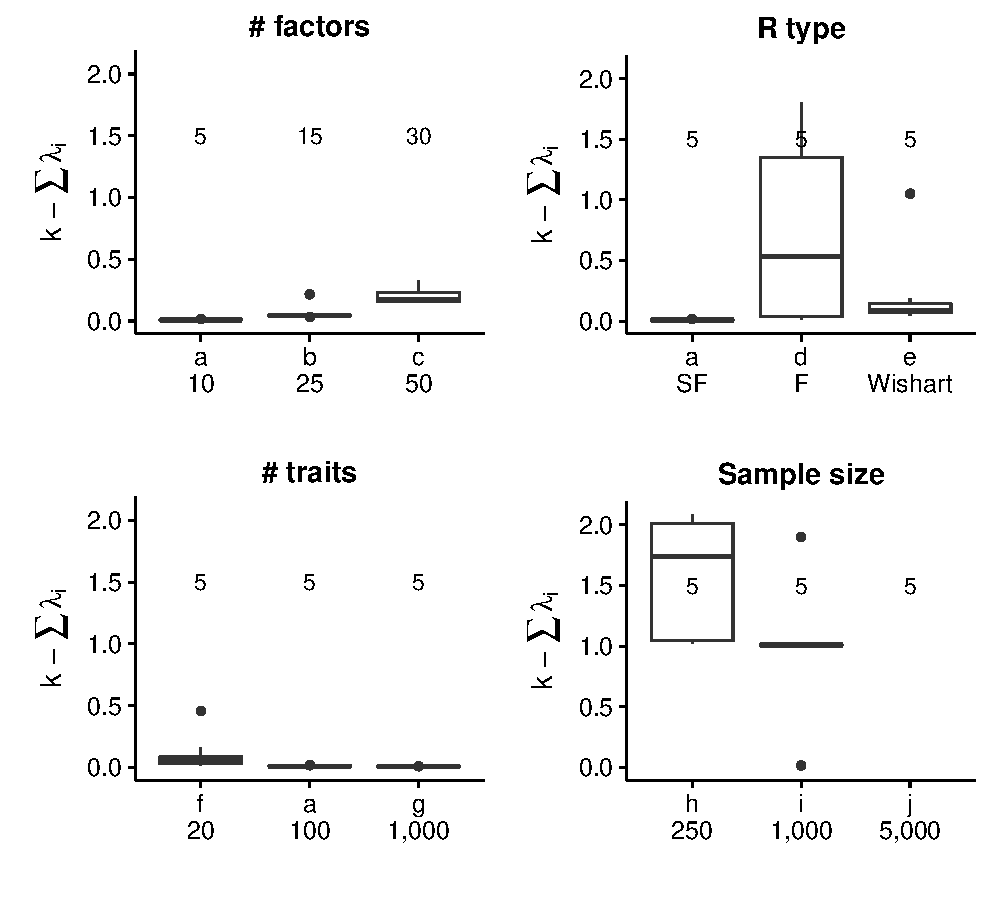
\includegraphics[width=5in]{Figures/K_dists_G.pdf}
\caption[Krzanowski substance comparison statistics for G by scenario]{ \textbf{The Bayesian genetic sparse factor model accurately estimates the dominant subspace of high-dimensional G matrices.} Each subplot shows the distribution of Krzanowski's statistics ($\sum \lambda_{s_i}$, \citeNP{Krzanowski:1979cx,Blows:2004ui}) calculated for posterior mean estimates of $\mathbf{G}$ across a related set of scenarios. Plotted values are $k - \sum \lambda_{s_i}$ so that statistics are comparable across scenarios with different subspace dimensions. On this scale, identical subspaces have a value of zero and values increase as the subspaces diverge. The value of $k$ used in each scenario is listed inside each boxplot. The difference from zero roughly corresponds to the number of eigenvectors of the true subspace missing from the estimated subspace. Different parameters were varied in each set of simulations as listed below each box. \textbf{A}. Increasing numbers of simulated factors. \textbf{B}. Different properties of the $\mathbf{R}$ matrix. ``SF": a sparse-factor form for $\mathbf{R}$, ``F": a (non-sparse) factor form for $\mathbf{R}$, ``Wishart": $\mathbf{R}$ was sampled from a Wishart distribution. \textbf{C}. Different numbers of traits. \textbf{D}. Different numbers of sampled individuals. Note that in scenarios \emph{h}-\emph{j}, factor $h^2$s ranged from 0.0 to 0.9. Complete parameter sets describing each simulation are described in Table~\ref{table:simulation_setup}.}
\label{fig:Krzanowski_G}
\end{center}
\end{figure}


\begin{figure}[b]
\begin{center}
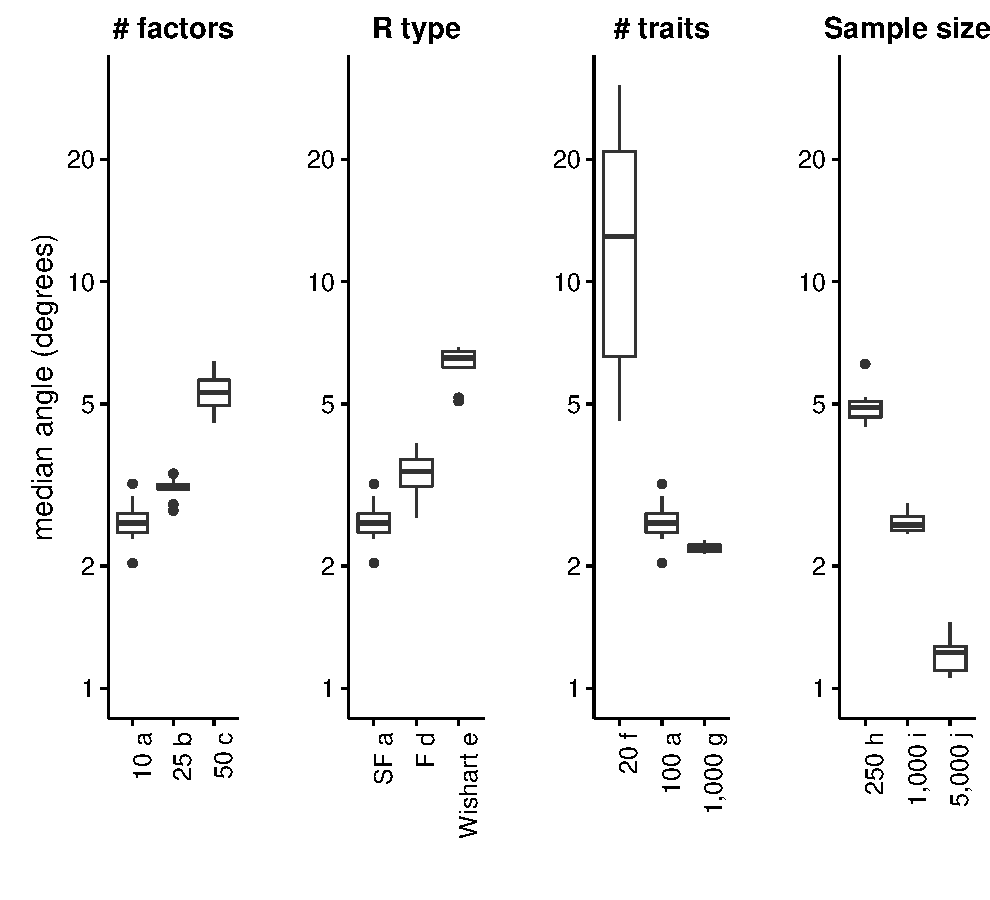
\includegraphics[width=5in]{Figures/factor_angles.pdf}
\caption[Error in latent factor trait loadings by scenario]{ \textbf{Latent factors were accurately recovered in most simulations.} The true factors in each simulation were matched to the most similar estimated factor by calculating the minimum vector angle between each true factor and an estimated factor. The median error angle across factors in each simulation is plotted. Boxplots show the distribution of median error angles by scenario. Two identical vectors have an angle of zero. Completely orthogonal vectors have an angle of 90. \textbf{A}. Increasing numbers of simulated factors. \textbf{B}. Different properties of the $\mathbf{R}$ matrix. \textbf{C}. Different numbers of traits. \textbf{D}. Different numbers of sampled individuals.}
\label{fig:factor_angles}
\end{center}
\end{figure}

\begin{figure}[b]
\begin{center}
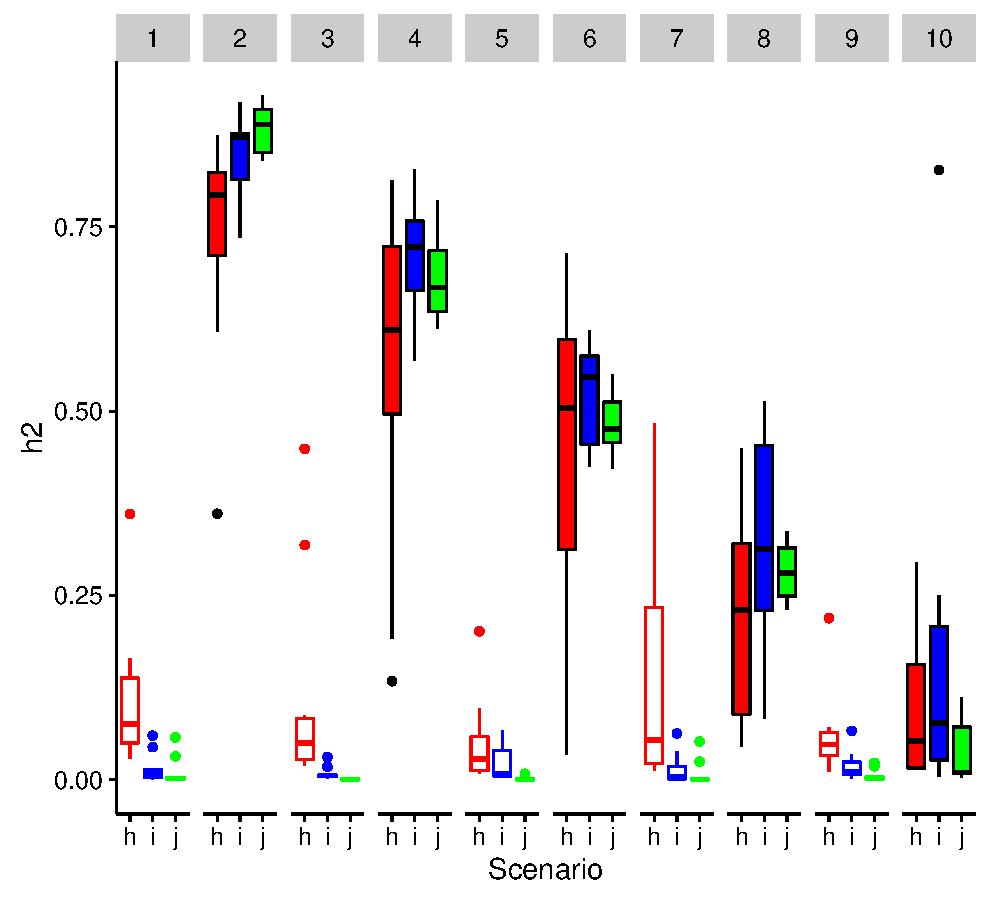
\includegraphics[width=5in]{Figures/factor_h2s.pdf}
\caption[Heritability of latent factors]{ \textbf{Latent factor heritabilities were accurately recovered.} Distributions of factor $h^2$ estimates for scenarios \emph{h}-\emph{j}. These scenarios differed in the number of individuals sampled. 10 factors were generated in each simulation and assigned $h^2$s between 0.0 and 0.9. After fitting our factor model to each simulated dataset,  the simulated factors were matched to estimated factors based on the trait-loading vector angles. Each boxplot shows the distribution of $h^2$ estimates for each simulated factor across 10 simulations. Note that the trait-loadings for each factor differed in each simulation; only the $h^2$ values remained the same. Thin horizontal lines in each column show the simulated $h^2_j$ values. Colors correspond to the scenario, and filled boxes/circles are used for factors with $h^2_j > 0$.}
\label{fig:factor_h2s_D}
\end{center}
\end{figure}


\begin{figure}[b]
\begin{center}
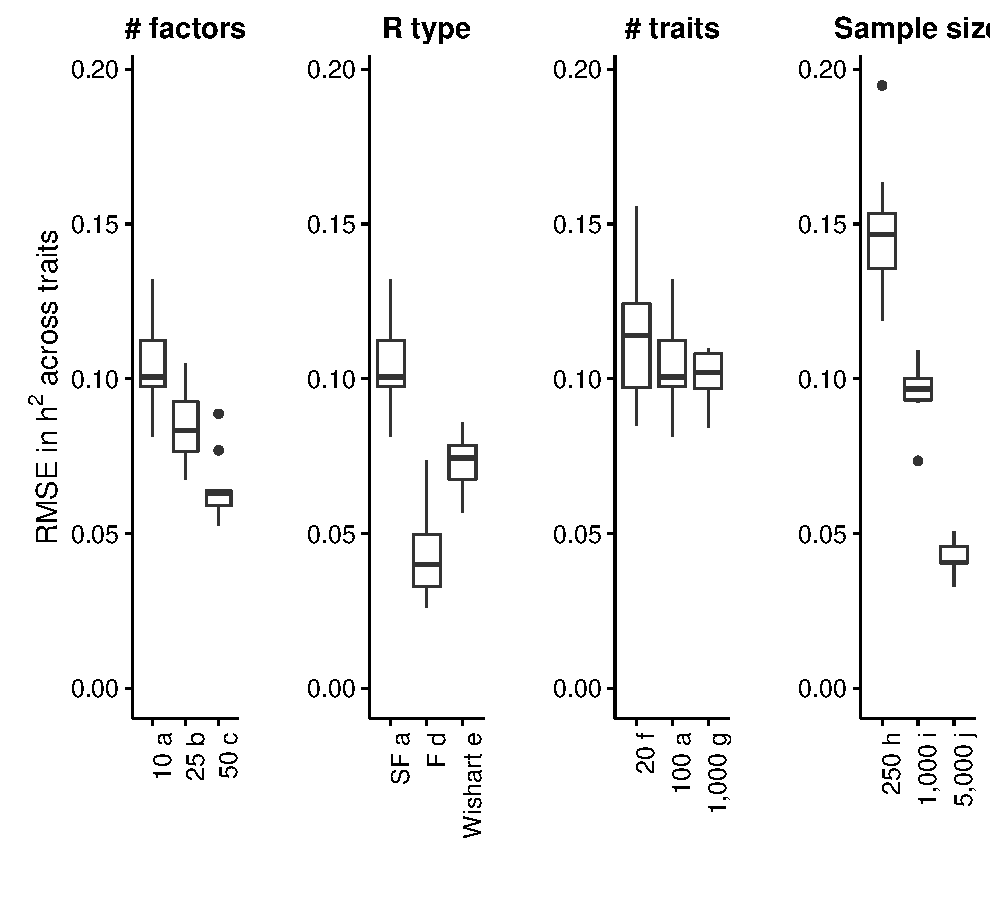
\includegraphics[width=5in]{Figures/RMSE.pdf}
\caption[Error in trait heritability]{ \textbf{Heritability estimates for each individual trait were accurate.} The heritability of each individual trait was estimated as $h^2_i = \mathbf{G}_{ii}/\mathbf{P}_{ii}$. RMSE $= \sqrt{\frac{1}{p}\sum\limits_{i=1}^p(\hat{h}^2_i - h^2_i)^2}$ was calculated for each simulation. Boxplots show the distribution of RMSE values for each scenario. \textbf{A}. Increasing numbers of simulated factors. \textbf{B}. Different properties of the $\mathbf{R}$ matrix. \textbf{C}. Different numbers of traits. \textbf{D}. Different numbers of sampled individuals. }
\label{fig:trait_h2s}
\end{center}
\end{figure}


%\begin{figure}[b]
%\begin{center}
%\includegraphics[width=6in]{Figures/Fitness_correlations_V3.pdf}
%\caption[Estimated G for Drosophila data]{ \textbf{Among-line covariance of gene expression and competitive fitness in Drosophila is modular.} \textbf{A-C} Genetic (among-line) architecture of 414 gene expression traits \cite{Ayroles:2009gd}. \textbf{A}. Posterior mean broad-sense heritabilities ($H^2$) for the 414 genes. \textbf{B}. Posterior mean genetic correlations among these genes. \textbf{C}. Posterior means and $95\%$ highest posterior density (HPD) intervals around estimates of genetic correlations between each gene and competitive fitness. For comparison, see Figure 7a of \citeN{Ayroles:2009gd}. \textbf{D-F}. Latent trait structure underlying gene expression covariances. \textbf{D} Posterior mean $H^2$ for each estimated latent trait. \textbf{E}. Posterior mean gene loadings on each latent trait. \textbf{F}. Posterior means and $95\%$ (HPD) intervals around estimates of genetic correlations between each latent trait and competitive fitness. The right-axis of panel \textbf{E}. groups genes into modules inferred using Modulated Modularity Clustering \cite{Stone:2009jx,Ayroles:2009gd}.}
%\label{fig:Fitness_G}
%\end{center}
%\end{figure}

%Supplemental Figures
\setcounter{figure}{0}
\makeatletter 
\renewcommand{\thefigure}{S\@arabic\c@figure}
\begin{figure}[b]
\begin{center}
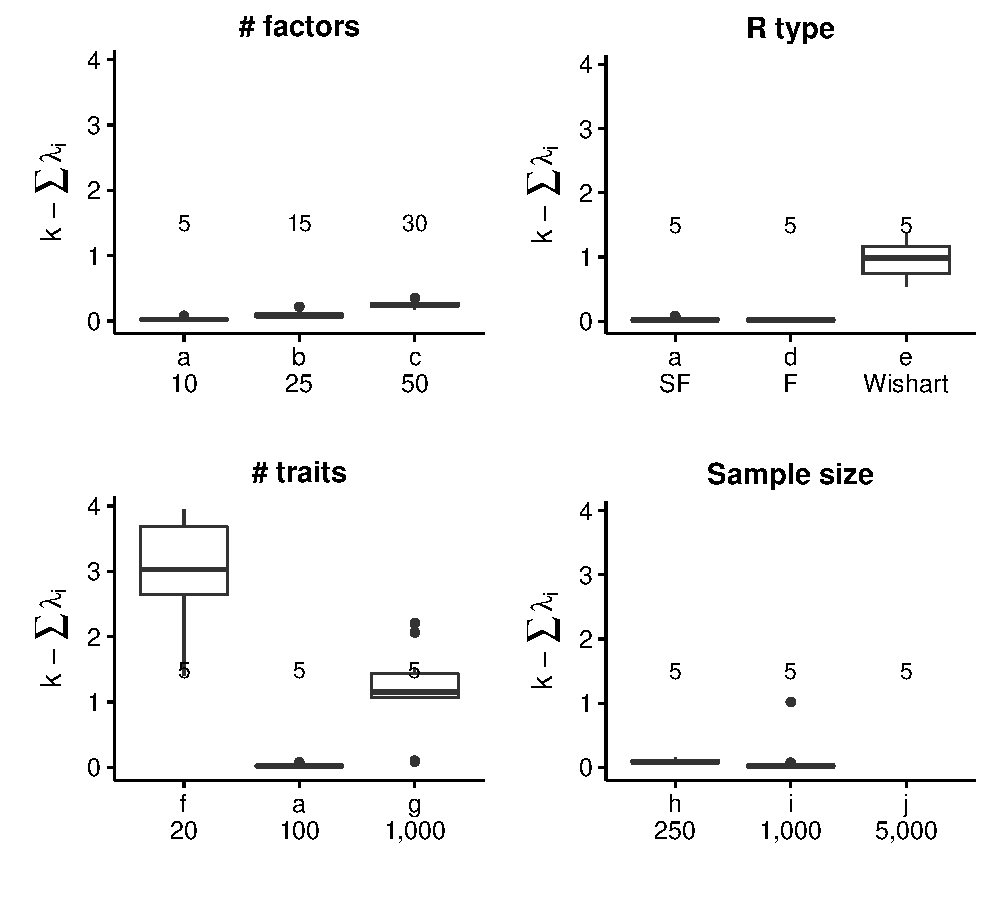
\includegraphics[width=5in]{Figures/K_dists_P.pdf}
\caption[Krzanowski substance comparison statistics for P by scenario]{ \textbf{$\mathbf{P}$-matrix subspaces were accurately recovered.} This figure is identical to Figure 1 but for $\mathbf{P}$. Each subplot shows the distribution of Krzanowski's statistics ($\sum \lambda_{s_i}$) calculated for posterior mean estimates of $\mathbf{P}$ across a related set of scenarios. The value of $k$ used in each scenario is listed inside each boxplot. The parameter varied in each set of simulations is described at the bottom. (A) Increasing numbers of simulated factors. (B) Different properties of the $\mathbf{R}$ matrix. ``SF": a sparse-factor form for $\mathbf{R}$, ``F": a (non-sparse) factor form for $\mathbf{R}$, ``Wishart": $\mathbf{R}$ was sampled from a Wishart distribution. In scenario \emph{e}, the residual matrix did not have a factor form. Therefore, we chose $k=19$ for the phenotypic covariance matrix because the corresponding eigenvectors each explained $>1\%$ of total phenotypic variation. (C) Different numbers of traits. (D) Different numbers of sampled individuals. Complete parameter sets describing each simulation are described in Table 1.}
\label{fig:Krzanowski_P}
\end{center}
\end{figure}


\begin{figure}[b]
\begin{center}
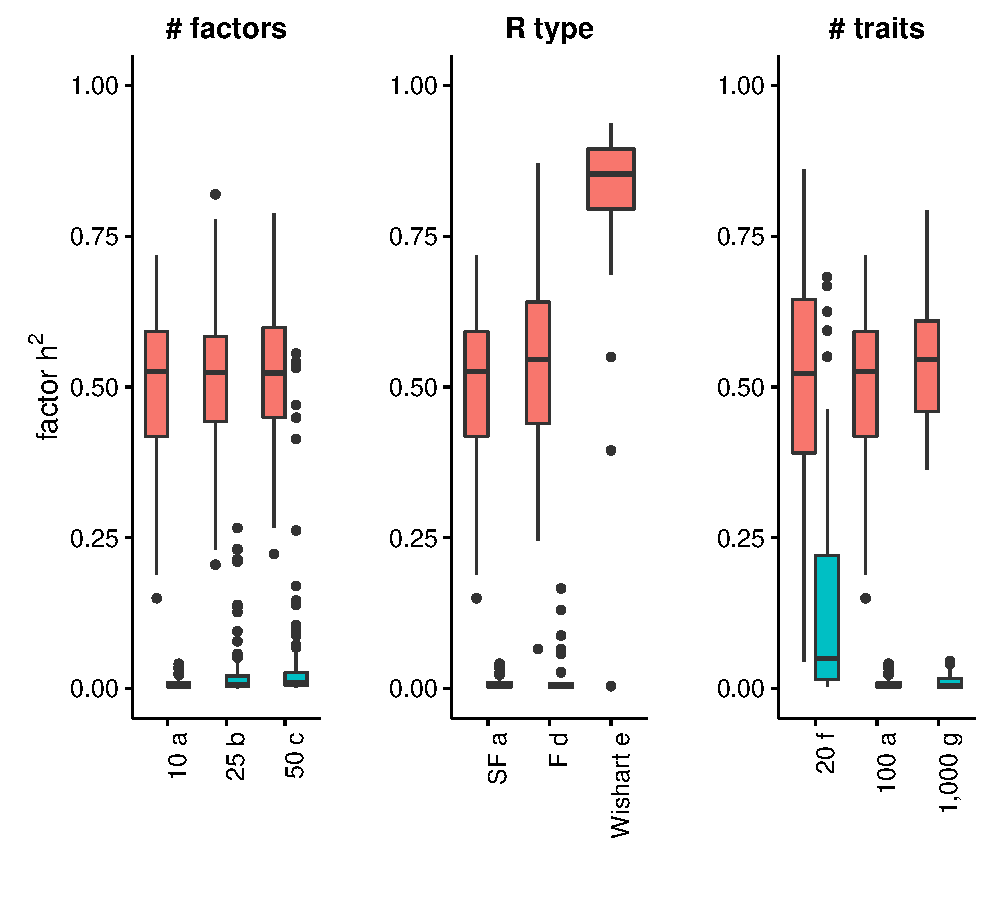
\includegraphics[width=5in]{Figures/factor_h2.pdf}
\caption[Heritability of latent factors]{ \textbf{Latent factor heritabilities were accurately recovered.} Distributions of factor $h^2$ estimates by simulation scenario. Each simulated factor was matched to the estimated factor with most similar trait-loadings as in Figure~\ref{fig:factor_h2s_D}. Thin horizontal lines in each column show the simulated $h^2_j$ values. Each simulated factor was assigned $h^2 = 0.0$ (black) or $0.5$ (red), except in scenario \emph{e} where all five factors were assigned $h^2 = 1$ (red). $h^2$ estimates are grouped across all 10 simulations of each scenario. (A) Increasing numbers of simulated factors. (B) Different properties of the $\mathbf{R}$ matrix. (C) Different numbers of traits.}
\label{fig:factor_h2s_ABC}
\end{center}
\end{figure}


\end{document}